%%%%%%%%%%%%%%%%%%%%%%%%%%%%%%%%%%%%%%%%%%%%%%%%%%%%%%%%%%%%%%%%%%%%%%%%%%%%%%%%
%2345678901234567890123456789012345678901234567890123456789012345678901234567890
%        1         2         3         4         5         6         7         8

\documentclass[letterpaper, 10 pt, conference]{ieeeconf}  % Comment this line out
                                                          % if you need a4paper
%\documentclass[a4paper, 10pt, conference]{ieeeconf}      % Use this line for a4
                                                          % paper

\IEEEoverridecommandlockouts                              % This command is only
                                                          % needed if you want to
                                                          % use the \thanks command
\overrideIEEEmargins
% See the \addtolength command later in the file to balance the column lengths
% on the last page of the document



% The following packages can be found on http:\\www.ctan.org
%\usepackage{graphics} % for pdf, bitmapped graphics files
%\usepackage{epsfig} % for postscript graphics files
%\usepackage{mathptmx} % assumes new font selection scheme installed
%\usepackage{times} % assumes new font selection scheme installed
%\usepackage{amsmath} % assumes amsmath package installed
%\usepackage{amssymb}  % assumes amsmath package installed
\usepackage{graphicx}

\title{\LARGE \bf
CS4047: In-Course Assessment
}

%\author{ \parbox{3 in}{\centering Huibert Kwakernaak*
%         \thanks{*Use the $\backslash$thanks command to put information here}\\
%         Faculty of Electrical Engineering, Mathematics and Computer Science\\
%         University of Twente\\
%         7500 AE Enschede, The Netherlands\\
%         {\tt\small h.kwakernaak@autsubmit.com}}
%         \hspace*{ 0.5 in}
%         \parbox{3 in}{ \centering Pradeep Misra**
%         \thanks{**The footnote marks may be inserted manually}\\
%        Department of Electrical Engineering \\
%         Wright State University\\
%         Dayton, OH 45435, USA\\
%         {\tt\small pmisra@cs.wright.edu}}
%}

\author{Konrad Dryja - 51552177 \\
  University of Aberdeen \\
  \today% <-this % stops a space
}


\begin{document}



\maketitle
\thispagestyle{empty}
\pagestyle{empty}


%%%%%%%%%%%%%%%%%%%%%%%%%%%%%%%%%%%%%%%%%%%%%%%%%%%%%%%%%%%%%%%%%%%%%%%%%%%%%%%%
\begin{abstract}

Lorem Ipsum

\end{abstract}


%%%%%%%%%%%%%%%%%%%%%%%%%%%%%%%%%%%%%%%%%%%%%%%%%%%%%%%%%%%%%%%%%%%%%%%%%%%%%%%%
\section{INTRODUCTION}

Bio-inspired computing is an ever-expanding area within computer science attempting to apply concepts that we observe in nature and in living organisms to modern algorithms in order to improve their efficiency and accuracy. The combination of efforts by scientists from different departments - such as biology (Genetic Algorithms) or sociology (Particle Swarm Optimisation) - enabled current techniques to learn from their mistakes and adapt to the changing circumstances \& environment. I strongly believe that introduction of such methods into our company would help us tackle problems such as stock prediction \cite{gunasekaran2011evaluation} or improving our current Machine Learning efforts - with the ultimate target of increasing the profit potential. In this report, I would like to bring our attention to two of the most common approaches: Artificial Immune Systems and Artificial Neural Networks, where I will explain the potential application and how useful they could be for our business.

\section{ARTIFICIAL IMMUNE SYSTEM}

Artificial Immune System (AIS) draws directly from biology of humans' (and not only) immune systems - organism's first line of defence against unwanted cells or viruses. The exact details and biological explanation behind those concepts can get incredibly complex very quickly, so for the sake of brevity, we can distinguish two major actors: antibodies (released by B / T cells) and antigens (the viruses). The main goal of antibodies is to identify and destroy to antigens - most importantly, the fight is usually a collective effort of the entire system, rather than of the individual cells. Moreover, one of the crucial concepts that carries over from biology into computing application is "self" and "not-self". The immune system should be able to distinguish between bodies belonging to the organism ("self") and the ones that haven't been recognized and thus should be eliminated ("not-self"). Finally, the detection itself is performed either via Clonal Selection or Negative Selection. The former is based on cloning and mutating the bodies with the highest affinity and the later eliminates the bodies not fulfilling determined criteria (e.g., affinity, often presented as Euclidean distance to the nearest antibody).

\subsection{Applications}
One of the more beneficial examples to our business would certainly be stock prediction. Gunasekaran et al. \cite{gunasekaran2011evaluation} presented an experiment where AIS was deployed to measure the trends and fluctuations on Bombay stock exchange. By feeding data for the year of 2009, the scientists were able to predict with a high accuracy the SENSEX Index for the year of 2010 (Root Mean Square Error of 103.106). While constructing the model, various indicators were used, such as Money Flow Index or Simple Moving Average. The study was researching the ultimate error difference between application of AIS and ANN - the former having achieved better results. Figure \ref{fig:stock} shows the exact difference between the actual SENSEX index for Bombai stock exchange, index predicted by AIS and index predicted by ANN. \newline
\begin{figure}[h!]
  \centering
  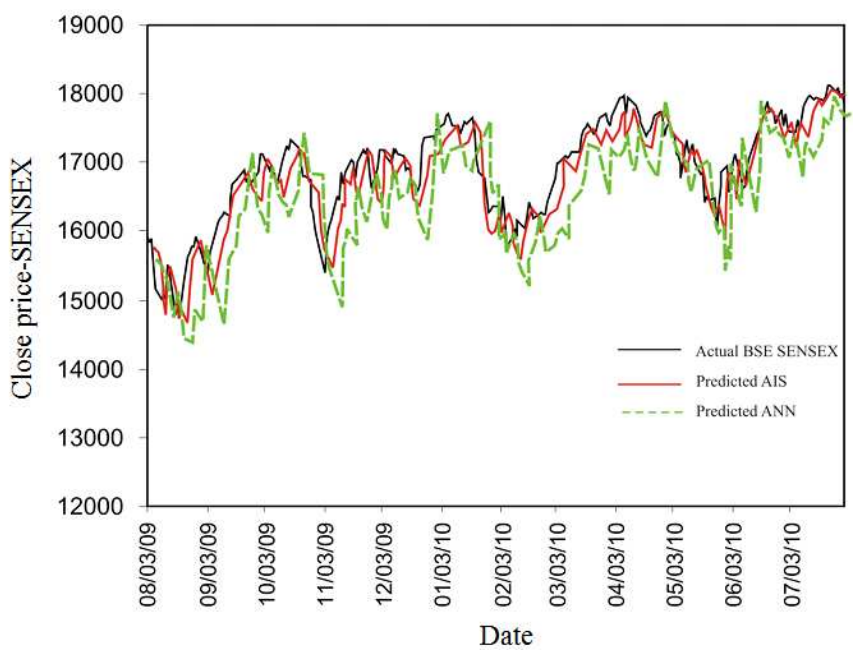
\includegraphics[width=0.4\textwidth]{graph}
  \caption{Comparison of AIM and ANN for stock prediction \cite{gunasekaran2011evaluation}}
  \label{fig:stock}
\end{figure}
Brabazon et al. \cite{brabazon2006biologically} also describes how Negative Selection can be used to determine set of companies that are due to fail and which ones will remain stable. In that particular scenario, "self" can be defined as healthy companies, whereas detectors would be build up from the historical financial data. Then, through the process of selection based on affinity to the detectors, a new set would be detected. Finally, all companies inside "not-self" set would be determined as failing or about to fail. This again could be utilised during decision process for investments. 


\subsection{Strengths aim at 100 words} 
Detectors hold the memory of previous 

The ability of 

\subsection{Weaknesses aim at 100 words}
Considering the example showing detection of failing companies - which utilizes the negative selection algorithm - one of the biggest challenges would be to handle the ever-growing set of "self", that is the number of companies is going to keep increasing, thus making this task more and more computationally expensive - as presented in the book \cite{brabazon2006biologically}.

Additionally, Timmis argues \cite{timmis2004overview} there is no precise field or application which AIM were designed for. This can be seen as both advantage and disadvantage, as it can be applied to a wider range of problems, al

\section{Artificial Neural Networks 150 words}
Lorem ipsum

\subsection{Applications aim at 150 words}
Lorem ipsum

\subsection{Strengths aim at 100 words}
Lorem ipsum

\subsection{Weaknesses aim at 100 words}
Lorem ipsum



\section{COMBINATIONS - aim at 150 words}

As useful individual methods are, the combination of different bio-inspired computation methods allows for even more powerful and precise machine learning paradigms. One of the most prominent examples being NeuroEvolution of Augmenting Topologies (NEAT) \cite{stanley2002evolving} presented by researches at University of Texas at Austin. The technique combines genetic algorithms along with artificial neural networks, allowing the latter to evolve and change it's layout (such as number and location of particular nodes in various layers across the network). That way the ANN can adapt and evolve according to the outside factors. Brabazon et al. Proposed applications 

\section{CONCLUSIONS - aim at 200 words}

Lorem ipsum\cite{gunasekaran2011evaluation}

\addtolength{\textheight}{-12cm}   % This command serves to balance the column lengths
                                  % on the last page of the document manually. It shortens
                                  % the textheight of the last page by a suitable amount.
                                  % This command does not take effect until the next page
                                  % so it should come on the page before the last. Make
                                  % sure that you do not shorten the textheight too much.

%%%%%%%%%%%%%%%%%%%%%%%%%%%%%%%%%%%%%%%%%%%%%%%%%%%%%%%%%%%%%%%%%%%%%%%%%%%%%%%%



%%%%%%%%%%%%%%%%%%%%%%%%%%%%%%%%%%%%%%%%%%%%%%%%%%%%%%%%%%%%%%%%%%%%%%%%%%%%%%%%



%%%%%%%%%%%%%%%%%%%%%%%%%%%%%%%%%%%%%%%%%%%%%%%%%%%%%%%%%%%%%%%%%%%%%%%%%%%%%%%%

\bibliographystyle{unsrt}
\bibliography{refs}

\end{document}

